\documentclass[12pt,a4paper]{ctexart}

% 第一至四问统一内容草稿的唯一当前入口，不是正式论文 paper/paper.tex。
% 草稿按论文正文版式编排；摘要留到四问完成后的最后阶段撰写。
\usepackage{amsmath,amssymb}
\usepackage{booktabs,longtable,array}
\usepackage{graphicx}
\usepackage{fontspec}
\usepackage[margin=2.5cm,headheight=15pt]{geometry}
\usepackage{fancyhdr}
\usepackage[hidelinks,hypertexnames=false]{hyperref}
\usepackage{caption}
\usepackage{cite}
\usepackage{enumitem}
\usepackage{float}
\usepackage{setspace}
\usepackage{titlesec}
\usepackage[section]{placeins}

\singlespacing
\setkeys{Gin}{width=\linewidth,keepaspectratio}
\providecommand{\tightlist}{\setlength{\itemsep}{0pt}\setlength{\parskip}{0pt}}

\setmainfont[
  Path=C:/Windows/Fonts/,
  UprightFont=times.ttf,
  BoldFont=timesbd.ttf,
  ItalicFont=timesi.ttf,
  BoldItalicFont=timesbi.ttf
]{Times New Roman}
\captionsetup{font=small,labelfont=bf}

\setcounter{secnumdepth}{4}
\renewcommand{\theparagraph}{\thesubsubsection.\arabic{paragraph}}
\titleformat{\section}{\centering\heiti\fontsize{14pt}{16pt}\selectfont}{\thesection}{1em}{}
\titlespacing{\section}{0pt}{12pt}{12pt}
\titleformat{\subsection}{\heiti\fontsize{12pt}{14pt}\selectfont}{\thesubsection}{1em}{}
\titlespacing{\subsection}{0pt}{6pt}{6pt}
\titleformat{\subsubsection}{\heiti\fontsize{12pt}{14pt}\selectfont}{\thesubsubsection}{1em}{}
\titlespacing{\subsubsection}{0pt}{6pt}{6pt}
\titleformat{\paragraph}[block]{\heiti\fontsize{12pt}{14pt}\selectfont}{\theparagraph}{1em}{}
\titlespacing{\paragraph}{1em}{6pt}{6pt}

\pagestyle{fancy}
\fancyhf{}
\renewcommand{\headrulewidth}{0pt}
\fancyfoot[C]{\thepage}

\hypersetup{
  pdftitle={第一至四问统一内容草稿（非正式论文）},
  pdfsubject={内部审阅稿，不作为正式提交论文}
}

\begin{document}

\begin{center}
{\heiti\fontsize{16pt}{19pt}\selectfont
乙醇偶合制备 C4 烯烃的实验关系分析与条件优化}
\end{center}
\vspace{18pt}

\section{问题重述}\label{sec:restatement}

\subsection{问题背景}

C4 烯烃是重要的化工原料。在乙醇偶合制备 C4 烯烃的过程中，催化剂组合和反应温度
会改变乙醇转化率及 C4 烯烃选择性。前者表示参与反应的乙醇比例，后者表示 C4 烯烃
在全部产物中的比例；二者共同决定 C4 烯烃收率。因此，评价实验条件时必须同时考察
转化率和选择性。

题目给出了21种催化剂组合在若干温度下的实验结果，以及350 ℃下某次实验在不同时刻
的测试结果。需要利用这些数据研究指标与温度的关系，比较催化剂组合和温度的影响，
选择收率较高的实验条件，并设计5次补充实验。

\subsection{问题提出}

本文需要解决以下四个问题：

\begin{enumerate}
\def\labelenumi{\arabic{enumi}.}
\tightlist
\item
  对附件 1 中每种催化剂组合分别研究乙醇转化率、C4 烯烃选择性与温度的关系，并
  分析附件 2 所给一次实验中各指标随时间的变化；
\item
  研究催化剂组合和温度对乙醇转化率、C4 烯烃选择性的影响；
\item
  选择使 C4 烯烃收率尽可能高的催化剂组合与温度，并在温度严格低于 350 ℃ 时
  另行选择；
\item
  在允许增加 5 次实验的条件下，给出具体实验安排及其理由。
\end{enumerate}

\section{问题分析}\label{sec:analysis}

\subsection{总体分析}

四个问题形成由现象认识到实验决策的递进关系。第一问关注单个催化剂组合内部的温度
关系及一次实验的时间变化；第二问转向组合与温度两类差异的比较；第三问把转化率和
选择性合成为收率，并据此选择实验条件；第四问再把前三问尚未解决的证据不足转化为
有限次数的补充实验。后问继承前问的数据口径和结论边界，但研究对象和所需证据不同，
不能机械套用同一模型。

\subsection{问题一分析}

第一问的两份附件具有不同的数据结构。附件1记录多个催化剂组合在若干固定温度下的
观测，任务是分别说明各组合内部的温度关系；附件2则记录同一次实验随时间的变化，
不能把多个时刻当作相互独立的重复实验。因此，两部分必须分别建立与其观测单位相符的
关系描述。

\subsubsection{附件1：各催化剂组合的温度关系}

每种组合的温度点较少，复杂曲线容易把个别波动解释成稳定规律；不同组合的配方和温度
覆盖又不完全相同，也不宜合并成一条总体曲线。为同时保留局部变化和总体方向，本文先
比较同一组合的相邻温度观测，再用简单线性关系概括其平均变化。该方法只描述各组合
已测温度范围内的经验关系，不承担连续温度预测或因果解释。

\subsubsection{附件2：一次实验的时间变化}

附件2的观测时刻间隔不等，变化量必须结合实际时间间隔解释。与此同时，各类产物
选择性共同构成产物份额，单类选择性的升降可能来自份额重新分配，不能彼此割裂。
因此，本文分别考察主要指标的时间变化和产物份额结构；反应路线文献只用于提出与现象
相容的可能机制，不作为本题具体机理的证明
\cite{aitchison1982,ho2016,moteki2016,sushkevich2017}。

\subsection{问题二分析}

第二问既要判断温度变化，也要比较催化剂组合，还要考察不同组合随温度变化的幅度是否
一致。
这三项任务的比较对象不同：温度影响应在同一组合内部判断，组合差异应在同一温度下
判断，而两者共同变化需要在前两类比较的基础上再作概括。

附件在不同温度下覆盖的组合并不完全相同。若直接比较各温度的全部记录，均值变化会
同时混入温度差异和样本组成变化。为保持比较对象一致，主体分析应使用组合覆盖相同的
温度记录，其他不完整温度只能在具有匹配观测的组合内作补充。同时，题目给出的每个
催化剂组合作为一个完整类别，现有数据不足以把组合差异归因于某个单一配方因素
\cite{searle1980}。

同组配对与同温比较能够回答具体方向和相对高低，但还不能统一衡量组合差异、温度差异
及未被简单相加关系解释的变化。因此，需要在可比数据上建立加和分解。由于每个实验
条件没有重复观测，未解释部分不能单独归因于组合与温度的共同作用或实验误差；模型只作描述性
分解，并通过保持比较结构的删减检查限定结论范围
\cite{nisttwoway,graphpadnorep}。

\subsection{问题三分析}

第三问要求在一般情景和严格低温情景下选择使 C4 烯烃收率尽可能高的条件。催化剂组合
是离散类别，各组合的温度观测又少且不完整。若直接拟合连续曲线再求极值，模型形式会
替代实验数据决定答案；若完全忽略内部缺测，又无法判断已有温度标签中的空白是否可能
改变推荐。

因此，本文把实测条件比较与缺测核查分开：正式推荐只在符合情景约束的真实观测中
产生，内部估计只用于检查缺测单元是否可能改变该推荐。辅助估计不得跨组合借用曲线、
超出组合自身实测范围或生成新配方，也不得以预测值替代实验事实。这样的分层使正式
答案的证据身份明确，同时保留对数据覆盖不足的必要检查。

\subsection{问题四分析}

第四问的目标不是用新增实验重复证明前三问，而是在5次预算内优先减少最影响条件选择的
不确定性。前三问暴露的数据不足可以归为三类：关键温度区间观测稀疏、最高观测缺少
独立重复、不同组合缺少新增同温条件下的直接比较。因此，实验设计既要补充局部温度
信息，也要兼顾可复现性和竞争组合比较，不能只按某个拟合模型的预测收率排序。

要刻画各组合在整个温度范围内的弯曲变化，即建立完整响应面，需要更多实验；本题的
催化剂组合又是不可随意拆分的离散类别。5次预算不足以同时确定全温区的曲线形态、
组合差异和随机误差。本文因而采用证据缺口驱动的局部增补：
先由前三问已经得到的结果明确每项未决问题，再为每次实验规定明确且可核查的职责。
具体缺口、实验条件和观测后的更新规则均在第四问模型建立与求解中给出
\cite{nistreplication,nistrsmcompare}。


\section{模型假设}\label{sec:assumptions}

\begin{enumerate}
\def\labelenumi{\arabic{enumi}.}
\item
  假设\textbf{附件中同一指标采用一致的测量定义和单位}，从而可以比较不同温度和
  不同催化剂组合下的记录。若实验批次采用了不可比的检测口径，本文的比较不再成立。
\item
  附件未记录进料波动、设备状态和催化剂表面变化，故假设\textbf{附件2的未记录实验
  条件在20---273 min内没有发生系统性改变}。这一假设使各时刻可以沿时间比较，但不能
  据此把观察到的变化唯一归因于催化剂失活。
\item
  为核查第三问中的内部缺测，假设\textbf{同一组合在相邻实测温度之间的收率可以作
  保形插值}，即可以用不额外制造局部振荡的平滑曲线连接相邻实测点。该条件只用于
  筛查缺测单元；预测值不作为真实观测，也不允许外推到组合自身实测范围之外。
\item
  设计第四问实验时，假设\textbf{新增实验沿用附件1对应组合的完整配方、装料方式和
  其余可控条件}，从而使新增结果可与原记录比较。337.5~℃是否可执行仍由设备控温能力
  决定，不属于本假设已经保证的条件。
\end{enumerate}

\section{符号说明}\label{sec:symbols}

本文统一使用表~\ref{tab:symbols} 所列符号；仅在局部使用的中间量，均在首次出现处说明。

\begin{table}[H]
\centering
\caption{主要符号及其含义}
\label{tab:symbols}
\small
\renewcommand{\arraystretch}{1.12}
\setlength{\tabcolsep}{6pt}
\begin{tabular}{
  >{\centering\arraybackslash}p{2.8cm}
  p{8.8cm}
  >{\centering\arraybackslash}p{2.8cm}}
\toprule
符号 & 含义 & 单位或取值 \\
\midrule
\(i,j\) & 催化剂组合编号、组合内按温度升序排列的观测序号 & 正整数 \\
\(n_i\) & 催化剂组合 \(i\) 的温度观测数 & 个 \\
\(T,t\) & 反应温度、实验时间 & ℃，min \\
\(X_i(T)\) & 组合 \(i\) 在温度 \(T\) 下的乙醇转化率 & \% \\
\(S_i(T)\) & 组合 \(i\) 在温度 \(T\) 下的 C4 烯烃选择性 & \% \\
\(Y_i(T)\) & 组合 \(i\) 在温度 \(T\) 下的 C4 烯烃收率 & \% \\
\(X_{ij},S_{ij},Y_{ij}\) & 上述三项指标在组合 \(i\) 第 \(j\) 个温度观测处的离散记号 & \% \\
\(\Delta X_{ij},\Delta S_{ij}\) & 相邻温度观测之间的转化率差和选择性差 & 百分点 \\
\(Z_{ij},\widehat Z_{ij}\) & 考察指标的观测值及其线性拟合值 & \% \\
\(a_i,b_i\) & 组合 \(i\) 的线性回归截距和斜率 & \%，\%/℃ \\
\(e_{ij},R_i^2\) & 线性回归残差和决定系数 & 百分点，无量纲 \\
\(v_j\) & 相邻时刻之间折算到每 10 min 的指标变化量 & 百分点 \\
\(P_k(t)\) & 时刻 \(t\) 第 \(k\) 类产物的选择性 & \% \\
\(r_A(t),r_H(t)\) & 乙醛、脂肪醇相对于 C4 烯烃的选择性份额比 & 无量纲 \\
\(y_{ij}\) & 共同温度分析中组合 \(i\) 在温度 \(j\) 下的考察指标 & \% \\
\(\mu\) & 相加模型中的总体均值 & \% \\
\(\alpha_i\) & 扣除温度总体差异后的组合偏差 & 百分点 \\
\(\beta_j\) & 温度平均偏差 & 百分点 \\
\(r_{ij}\) & 简单相加未解释变化 & 百分点 \\
\(D_{0}^{\mathrm{all}},D_{0}^{\mathrm{low}}\) & 第三问中的全部实测候选域和严格低温实测候选域 & 集合 \\
\(c_e,T_e\) & 第 \(e\) 次新增实验的催化剂组合和反应温度 & 组合，℃ \\
\(X_e,S_e,Y_e\) & 第 \(e\) 次新增实验测得的转化率、选择性和收率 & \% \\
\bottomrule
\end{tabular}
\end{table}

除特别说明外，本文用百分数表示比例，用``百分点''表示两个百分数的绝对差。例如，
选择性由 30\% 增至 35\% 时，其变化量为 5 个百分点。

\section{数据预处理}\label{sec:data}

本文把附件1中每个组合编号对应的整套实验条件视为一种催化剂组合，不拆分其中的
Co负载量、HAP质量和装料方式。附件1共有114条“催化剂组合—温度”记录，覆盖21种
组合，每种组合具有5至7个温度点。附件2包含20、70、110、163、197、240和273 min共7个
不等间隔时刻，每个时刻记录乙醇转化率及六类产物选择性。

预处理统一了百分数格式，检查了重复记录、缺失值和各组合的温度覆盖，并将整理后的
数据逐项与原附件核对。所有观测均予以保留。C4 烯烃收率按题目定义计算：

\begin{equation}
Y_i(T)=\frac{X_i(T)S_i(T)}{100}.
\tag{1}
\label{eq:c4-yield}
\end{equation}

式\eqref{eq:c4-yield}把乙醇参与反应的比例和目标产物在全部产物中的比例合并为统一
产出指标。该式
也说明，当转化率和选择性一升一降时，不能只依据其中一个指标判断收率变化。

\section{模型建立与求解}\label{sec:model}
\subsection{问题一：温度关系与时间变化}

本问分别处理附件1和附件2。对于附件1，本文用直线概括每种催化剂组合的平均温度
关系，并用相邻观测保留局部变化；对于附件2，本文按真实时间计算转化率、
选择性、收率和产物份额的变化。两部分均先给出计算关系，再报告结果和适用范围。

\subsubsection{附件 1：各催化剂组合的温度关系}

\paragraph{相邻温度下的实际变化}

对任一组合 \(i\)，将实际测试温度按
\(T_{i1}<T_{i2}<\cdots<T_{in_i}\) 排列。为保留已测条件之间的
真实变化，定义相邻温度指标差：

\begin{align}
\Delta X_{ij}&=X_i(T_{i,j+1})-X_i(T_{ij}), \tag{2}\label{eq:q1-adjacent-x}\\
\Delta S_{ij}&=S_i(T_{i,j+1})-S_i(T_{ij}). \tag{3}\label{eq:q1-adjacent-s}
\end{align}

当差值大于 0、等于 0 或小于 0 时，分别表示较高温度条件下指标上升、持平或局部
下降。式\eqref{eq:q1-adjacent-x}和式\eqref{eq:q1-adjacent-s}只连接附件中真实存在的相邻温度，不补造中间温度，也不把连线
解释为同一次连续升温过程。

各组合只使用自身实际存在的温度点，不补齐缺失温度。若全部相邻差值为正，则该指标在
已测相邻温度下均升高；若出现负值或零值，则记录相应温区和变化量。

以A5的转化率为例，250 ℃和275 ℃的观测值分别为14.7872\%和12.4240\%，所以该区间
转化率变化为：

\[
\Delta X_{\mathrm{A5}}=12.4240\%-14.7872\%=-2.3632\text{ 个百分点}.
\]

该负值直接说明A5在250---275 ℃之间出现局部下降。即使后续直线给出A5在全部已测范围
内的平均斜率为正，这一离散事实也必须保留。

图\ref{fig:q1-adjacent-map}汇总所有组合在相邻已测温度之间的实际变化。
\begin{figure}[H]
\centering
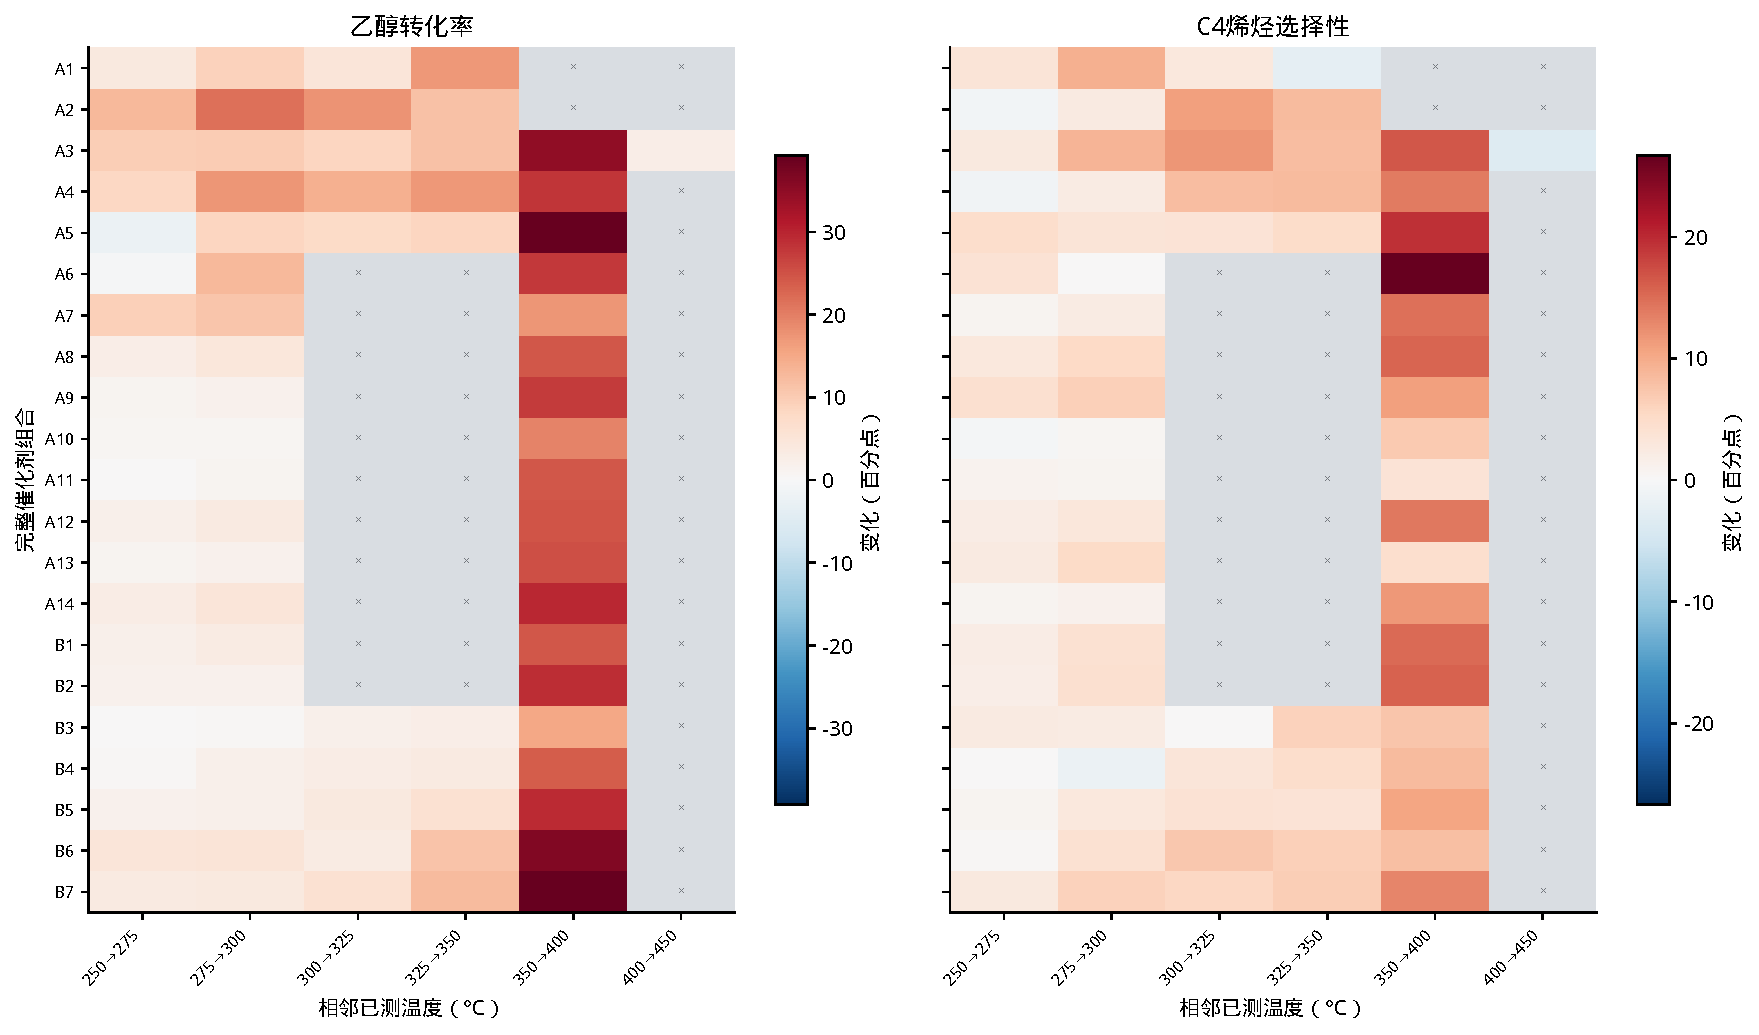
\includegraphics[width=0.82\linewidth]{../../output/q1/figures/02_adjacent_temperature_change_map.pdf}
\caption{各催化剂组合在相邻已测温度间的指标变化。暖色表示指标上升，冷色表示下降，
接近白色表示变化接近零，灰色叉号表示该组合不存在相应温度区间。}
\label{fig:q1-adjacent-map}
\end{figure}

暖色单元占多数，说明较高温度通常
对应较高的转化率和选择性；冷色或接近零的单元标出局部下降和持平。灰色叉号表示该
组合没有相应温区的记录。

\paragraph{每种组合的平均温度关系}

相邻差值能够显示局部变化，但不便于比较21种组合的平均升温幅度。因此，本文对每种
组合的转化率和选择性分别作一元最小二乘线性拟合：

\begin{align}
X_{ij}&=a_i^X+b_i^XT_{ij}+e_{ij}^X, \tag{4}\\
S_{ij}&=a_i^S+b_i^ST_{ij}+e_{ij}^S. \tag{5}
\end{align}

其中，$b_i^X$ 和 $b_i^S$ 分别表示温度每升高1 ℃时转化率和选择性的平均变化，
$e_{ij}$ 表示观测值与直线之间的差。为便于比较，结果统一报告 \(25b\)，即温度每升高
25 ℃时指标平均改变的百分点数。

对某一组合的某一个指标，统一记观测值为 $Z_{ij}$，样本均值为 $\bar T_i$ 和 $\bar Z_i$。使用最小二乘
法选择斜率，使全部观测点到直线的纵向偏差平方和最小。斜率和截距分别为：

\begin{align}
b_i&=\frac{\sum_j(T_{ij}-\bar T_i)(Z_{ij}-\bar Z_i)}
{\sum_j(T_{ij}-\bar T_i)^2}, \tag{6}\label{eq:q1-ols-slope}\\
a_i&=\bar Z_i-b_i\bar T_i. \tag{7}\label{eq:q1-ols-intercept}
\end{align}

将实际温度代入直线得到拟合值 \(\widehat Z_{ij}=a_i+b_iT_{ij}\)，残差为
\(e_{ij}=Z_{ij}-\widehat Z_{ij}\)。式\eqref{eq:q1-ols-slope}直接使用温度数值，因此能够处理不同的
温度间隔。

为说明直线对该组观测的概括程度，计算决定系数：

\begin{equation}
R_i^2=1-\frac{\sum_j e_{ij}^2}{\sum_j(Z_{ij}-\bar Z_i)^2}.
\tag{8}
\end{equation}

\(R_i^2\) 越接近1，观测点越接近拟合直线；数值较低时，平均斜率不能充分描述局部
形态。该指标只评价已测数据的拟合程度。

以 A1 为例，将其 5 个温度点分别代入式\eqref{eq:q1-ols-slope}和式\eqref{eq:q1-ols-intercept}，得到：

\[
X_{\mathrm{A1}}(T)=-84.0828+0.3332T,\qquad
S_{\mathrm{A1}}(T)=-3.2420+0.1544T.
\]

在A1的已测范围内，温度每升高25 ℃，转化率和 C4 烯烃选择性分别平均增加8.3297和
3.8590个百分点。截距只确定直线位置，不表示0 ℃时的实际指标。其余20种组合均按
相同步骤独立拟合。

\paragraph{斜率方向的逐点删除检验}

为判断斜率方向是否由单个观测主导，本文依次删除每个温度点并重新拟合。设删除第
\(j\) 个观测后的斜率为 \(b_{i,-j}\)，比较它与完整数据斜率 \(b_i\) 的符号：

\begin{equation}
\operatorname{sign}(b_{i,-j})=\operatorname{sign}(b_i).
\tag{9}\label{eq:q1-loo-sign}
\end{equation}

若所有删点结果都满足式\eqref{eq:q1-loo-sign}，则平均方向不依赖某一个观测。附件1的两个指标共进行
228次删点拟合；该检验只检查斜率方向，不用于判断曲线是否严格线性。

\paragraph{各组合关系的直接回答}

对转化率建立的21个线性关系均具有正斜率。按25 ℃换算后，转化率平均增加
3.2828---16.5740 个百分点。相邻差分进一步显示，19 种组合在全部相邻
已测条件下均上升，A5 和 A6 在 250---275 ℃ 间分别下降 2.3632 和 0.6084 个百分点。
因此，转化率的总体方向为正，但不能把 A5、A6 写成所有温度区间均严格增加。

对C4 烯烃选择性建立的21个线性关系同样均具有正斜率。温度每升高25 ℃，选择性平均
增加 1.2918---6.5299 个百分点。15 种组合在
全部相邻条件下均上升，其余组合存在以下局部例外：A2、A4、A10 在 275 ℃ 时低于
250 ℃；A1、A3 在最高测试温度低于前一个温度；B4 在 250---275 ℃ 持平，随后在
300 ℃ 出现下降。

A3 的转化率在 400---450 ℃ 间增加 2.6963 个百分点，而选择性下降 3.53 个百分点。
这一反向变化说明，更多乙醇参与反应并不保证目标产物所占比例同步提高，转化率和
选择性必须分别建模，并在后续收率分析中重新合并。

42组关系的 \(R^2\) 为0.7421---0.9988，最低值出现在A10的 C4 烯烃选择性关系。
228次删点拟合均未改变斜率方向，说明平均正向关系不由单个观测决定。图
\ref{fig:q1-linear-summary}把每组的斜率、\(R^2\) 和局部例外放在一起比较。

\begin{figure}[H]
\centering
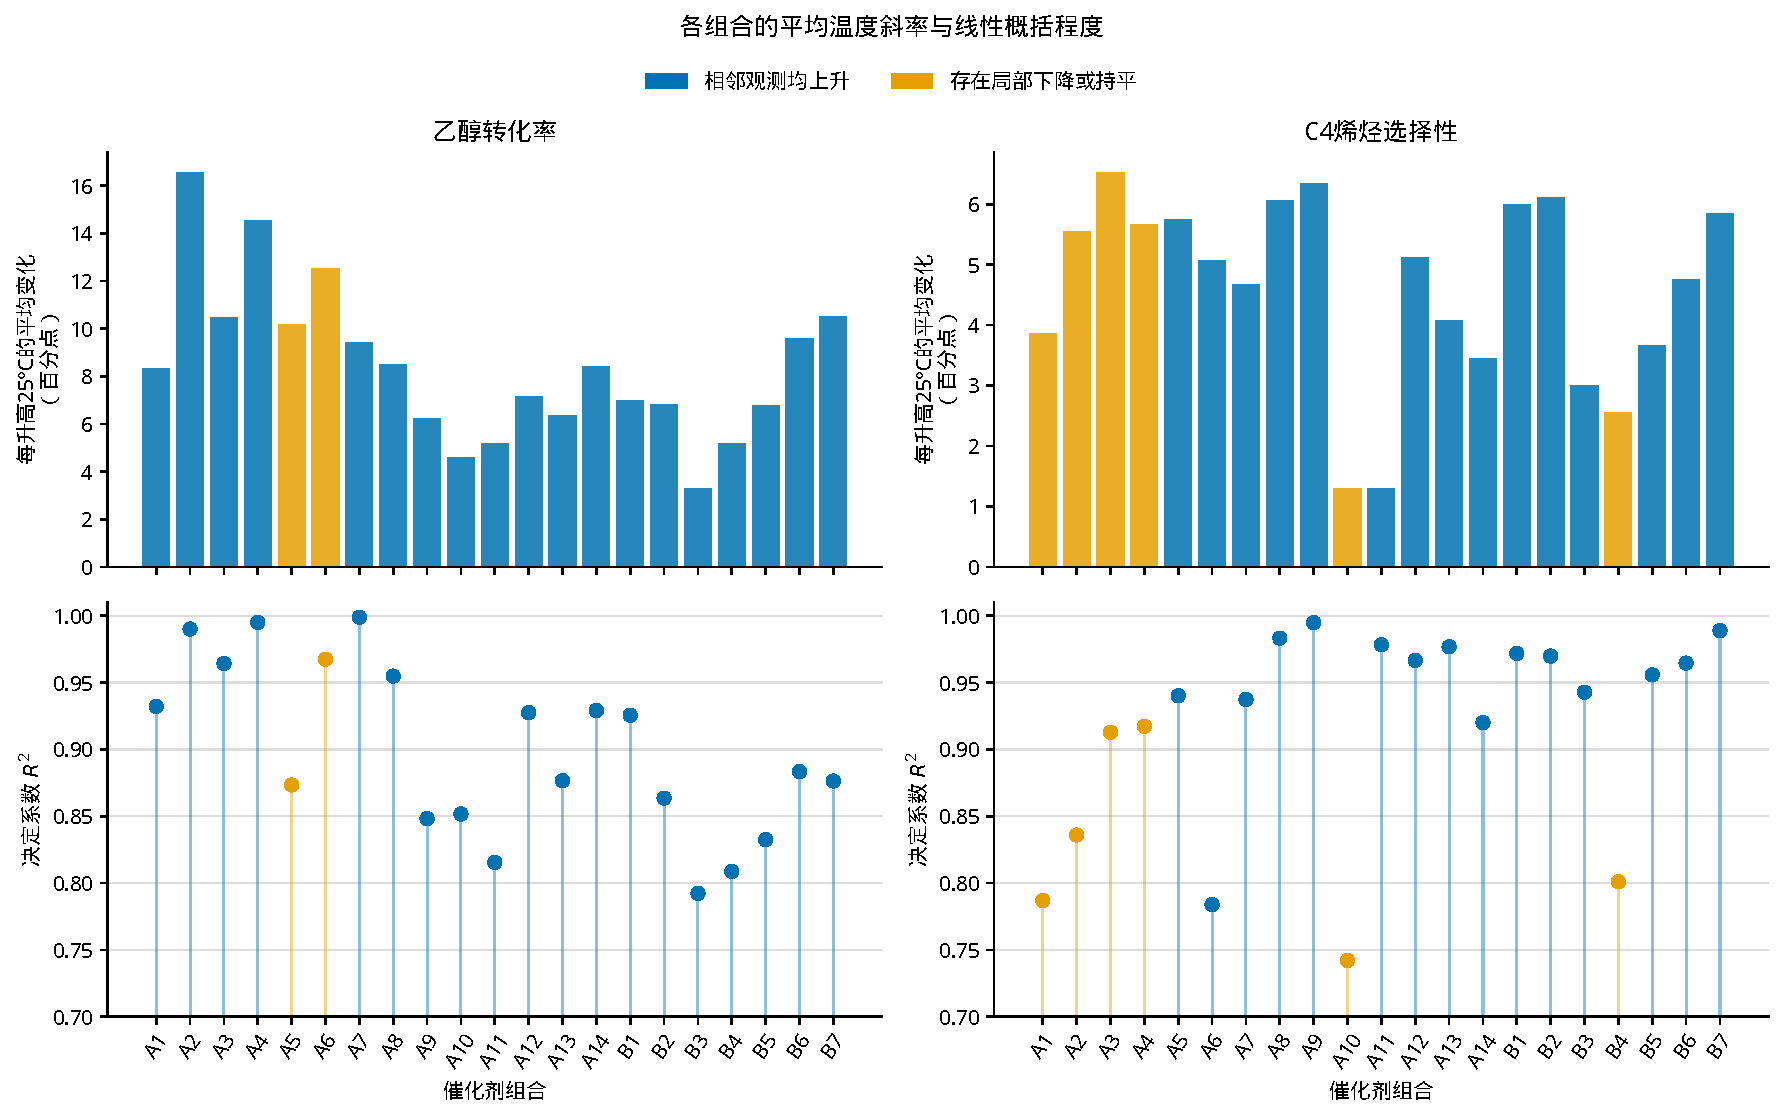
\includegraphics[width=\linewidth]{../../output/q1/figures/05_attachment1_linear_summary_diagnostics.pdf}
\caption{各催化剂组合在已测范围内的平均温度斜率与决定系数。上排分别给出乙醇转化率
和 C4 烯烃选择性每升高 25 ℃的平均变化量，下排给出对应 \(R^2\)。橙色表示该组合
至少存在一个局部下降或持平区间，蓝色表示全部相邻观测均上升。}
\label{fig:q1-linear-summary}
\end{figure}

该图显示，42条拟合直线的斜率均为正，但不同组合的斜率和
拟合程度差异明显。以A10为例，其选择性斜率为正，\(R^2=0.7421\)，但250---275 ℃
间实际下降，因此应描述为“平均正向，局部下降”。

综合42组结果，13种组合的两个指标在全部相邻温度下均升高；其余8种组合至少有一个
指标出现局部下降或持平。由此，第一问对各组合的回答统一为两类：“平均正向且无已测
局部例外”或“平均正向并伴随具体局部例外”。该结论限于各组合的已测温度范围。

\paragraph{附件 1 的计算一致性检验}

独立程序重新读取附件1，复算42组斜率、决定系数、相邻温度差和228次删点斜率，所得
结果与正文一致。该复算验证了计算过程，但现有数据仍不足以确定精确转折点或预测未测
温度。

\subsubsection{附件 2：一次实验的时间变化}

\paragraph{时间变化与稳定性判断}

设附件 2 时刻 t 的乙醇转化率、C4 烯烃选择性和收率分别为 X(t)、S(t) 和 Y(t)。
由于 7 个时刻间隔不等，所有变化速度均按真实分钟数计算。对总体下降方向清晰的转化率
和收率，建立只适用于 20---273 min 已观测区间的简单时间关系：

\begin{align}
X(t)&=\alpha_X+\beta_Xt+\varepsilon_X, \tag{10}\label{eq:q1-time-x}\\
Y(t)&=\alpha_Y+\beta_Yt+\varepsilon_Y. \tag{11}\label{eq:q1-time-y}
\end{align}

C4 烯烃选择性只在较窄范围内波动，因而用取值范围和首末变化描述；转化率和收率具有
清楚的下降趋势，因而再用式\eqref{eq:q1-time-x}和式\eqref{eq:q1-time-y}概括其平均变化速度。这里的``稳定''仅指
指标在本次观测时段内是否围绕近似固定水平小幅波动，不代表催化剂具有长期稳定性。

计算时，先由题给关系 \(Y(t)=X(t)S(t)/100\) 求出各时刻的 C4 烯烃收率。由于相邻观测
之间相隔 33---50 min，不能直接比较相邻差值，故将变化量统一换算为每 10 min 的变化：

\begin{align}
\Delta Z_j&=Z(t_{j+1})-Z(t_j),\notag\\
v_j&=\frac{10\Delta Z_j}{t_{j+1}-t_j}.
\tag{12}\label{eq:q1-time-change}
\end{align}

式\eqref{eq:q1-time-change}使不同长度的时间区间可以直接比较。再以真实时间 \(t\) 为自变量进行最小二乘
回归，并报告 \(10\beta\)，即每 10 min 的平均变化量。

7 个时刻的转化率由 43.5474\% 总体降至 29.9060\%，收率由 17.3754\% 总体降至
11.6753\%。两项指标均有清晰下降主线。C4 烯烃选择性则先降、后升、再波动，首末仅相差
0.86 个百分点。
因此，前两项用直线概括平均速度，选择性则保留实际范围和逐时刻变化。

\[
\widehat X(t)=42.6709-0.05276t,\qquad
\widehat Y(t)=16.5297-0.01989t .
\]

上述两式只概括 20---273 min 内的平均趋势。其中截距用于确定直线位置，不解释为
反应开始时刻的真实数值。

图\ref{fig:q1-time-regression}比较实际观测与20---273 min内的线性概括。
\begin{figure}[H]
\centering
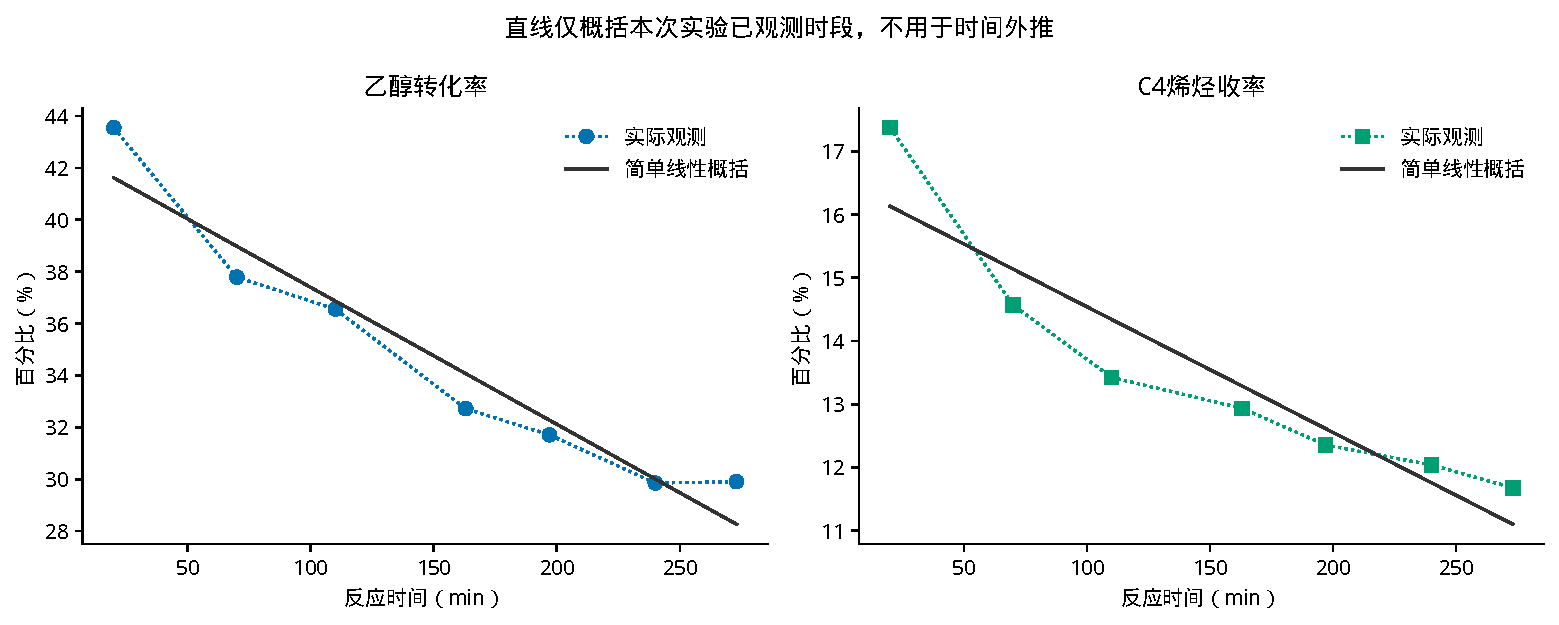
\includegraphics[width=0.90\linewidth]{../../output/q1/figures/06_attachment2_limited_linear_summaries.pdf}
\caption{附件 2 中乙醇转化率和 C4 烯烃收率的实际观测与线性概括。点线为实际观测，
黑色实线为 20---273 min 区间内的一元线性回归结果。}
\label{fig:q1-time-regression}
\end{figure}

由图可见，20---273 min 内乙醇转化率由 43.5474\% 降至 29.9060\%，下降
13.6414 个百分点；C4 烯烃收率由 17.3754\% 降至 11.6753\%，下降 5.7001 个百分点。
线性概括给出的平均速度分别为每 10 min 下降 0.5276 和 0.1989 个百分点，对应 $R^2$
分别为 0.9329 和 0.8575。实际点在前期下降较快、后期趋缓，且转化率在 240---273 min
回升 0.0518 个百分点，所以两条直线不能代替各时刻的真实变化。

C4 烯烃选择性由 39.90\% 变为 39.04\%，全过程位于 36.72\%---40.32\% 之间。与转化率和
收率的明显下降相比，选择性只在较小区间波动，表明本次实验中收率下降主要伴随乙醇
转化率降低，而不是由 C4 烯烃选择性持续下降造成。按上述判据，本次实验的选择性相对
稳定，但转化率和收率存在明显向下漂移，因而不能把整个反应表现概括为稳定。

\paragraph{产物份额的重新分配}

对每个时刻 t，六类产物选择性满足：

\begin{equation}
\sum_{k=1}^{6}P_k(t)=100\%.
\tag{13}\label{eq:q1-composition-sum}
\end{equation}

六类选择性合计为 100\%，所以它们表示产物组成中的相对份额。一类份额上升时，其他
类别的合计份额必然下降；这里研究的是产物组成如何变化，而不是六类产量各自如何变化。

除逐类比较首末份额外，再以C4 烯烃选择性为共同参照，定义：

\begin{align}
r_A(t)&=\frac{\text{乙醛选择性}}{\text{C4 烯烃选择性}},\notag\\
r_H(t)&=\frac{\text{C4---C12 脂肪醇选择性}}{\text{C4 烯烃选择性}}.
\tag{14}
\end{align}

\(r_A\) 和 \(r_H\) 分别比较乙醛、C4---C12 脂肪醇与 C4 烯烃的相对份额。前者增大
表示乙醛相对增多，后者减小表示脂肪醇相对减少；这两个比值不代表反应速率或直接转化。

图\ref{fig:q1-product-shares}同时展示六类产物份额和两项相对份额比的时间变化。
\begin{figure}[H]
\centering
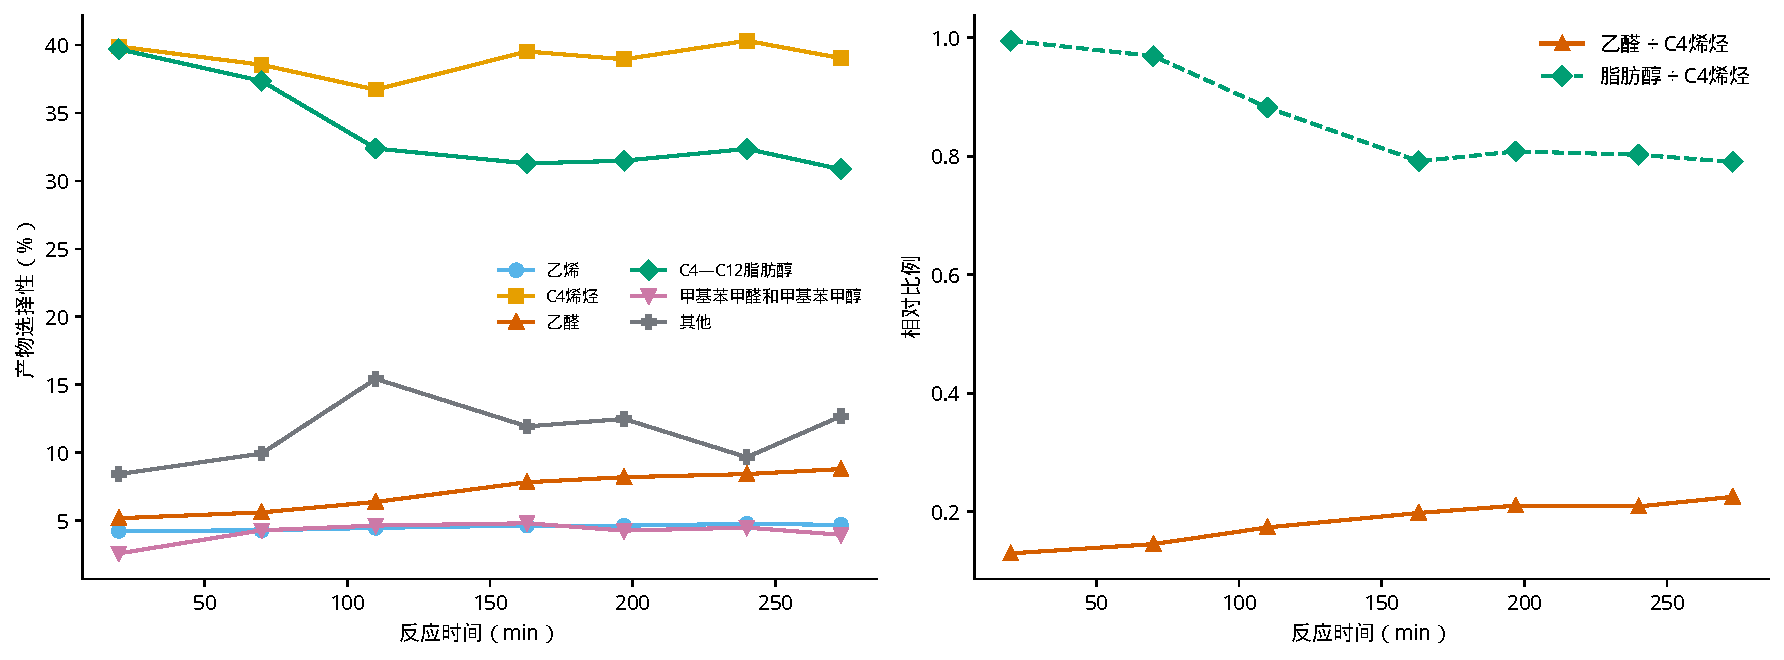
\includegraphics[width=0.90\linewidth]{../../output/q1/figures/03_attachment2_product_shares_and_ratios.pdf}
\caption{附件 2 中六类产物选择性及两项相对份额比随时间的变化。左图给出固定总和
份额的重新分配，右图给出乙醛和 C4---C12 脂肪醇相对 C4 烯烃的份额比。}
\label{fig:q1-product-shares}
\end{figure}

图中C4 烯烃选择性变化较小，但乙醛份额总体增加、
C4---C12 脂肪醇份额总体下降。为精确核对首末变化，表\ref{tab:q1-product-change}
列出 20 min 到 273 min 的百分点差。

\begin{table}[H]
\centering
\caption{附件 2 六类产物选择性的首末变化}
\label{tab:q1-product-change}
\begin{tabular}{lr}
\toprule\noalign{}
产物类别 & 首末变化/百分点 \\
\midrule\noalign{}
乙烯 & +0.45 \\
C4 烯烃 & −0.86 \\
乙醛 & +3.62 \\
C4---C12 脂肪醇 & −8.84 \\
甲基苯甲醛和甲基苯甲醇 & +1.37 \\
其他产物 & +4.26 \\
\bottomrule
\end{tabular}
\end{table}

增加项和减少项均合计 9.70 个百分点，与式\eqref{eq:q1-composition-sum}相符。
同期，乙醛与 C4 烯烃的份额比由 0.1296 升至 0.2252，C4---C12 脂肪醇与 C4 烯烃的
份额比由 0.9950 降至 0.7905。由此可见，即使 C4 烯烃选择性变化较小，产物内部结构
仍发生了明显调整，最突出的是脂肪醇份额下降而乙醛和其他产物份额上升。

已有研究表明，乙醛、较高碳数醇和烯烃可能处在相互衔接或竞争的反应路径中
\cite{ho2016,moteki2016,sushkevich2017}。这些研究为不同产物份额的同步变化提供了
可能的路径背景，但本题
缺少中间体示踪和反应速率数据，不能由此断言脂肪醇直接转化为 C4 烯烃。

\paragraph{测试现象的可能解释}

附件 2 中，乙醇转化率与 C4 烯烃收率同步下降，而 C4 烯烃选择性变化较小。这说明
目标产出降低主要来自乙醇转化率下降，而不是 C4 烯烃在产物中所占比例持续下降。若
催化剂的有效活性位在运行中减少或被覆盖，就可能出现这种``转化能力下降、主要产物
比例变化较小''的现象。

Yan 等在 Zn-Y/Beta 催化乙醇制丁二烯的实验中发现，含氧中间体继续缩合形成的物质会
逐渐覆盖活性位并导致催化剂失活 \cite{yan2018}。因此，活性位被覆盖可作为转化率下降
的一种可能解释。不过，该研究采用的催化剂和目标产物与本题不同，不能据此认定附件 2
中的催化剂发生了相同变化。

羟基磷灰石催化体系的研究还表明，乙醛可参与后续碳链增长，而生成较高碳数产物需要
继续经历缩合、氢转移和脱水等步骤 \cite{ho2016,moteki2016}。因此，若后续转化受到的
影响更强，乙醛的相对份额可能上升，较高碳数醇的份额可能下降。这与附件 2 的现象
相容，但选择性只是相对份额，不能据此判断乙醛的绝对生成量或证明产物之间直接转化。

时间序列还表现为前期下降较快、后期趋缓，最后一个区间轻微回升。这可能是体系逐渐
接近新的运行状态，也可能来自测量或操作波动。由于只有一次实验，且缺少催化剂表面
表征和重复测试，本文只把``活性位覆盖''和``后续转化受抑''列为可能机制，不作唯一
判断。

\paragraph{附件 2 的计算一致性检验}

独立程序复算了各时刻收率、时间斜率、两项份额比和六类选择性的首末变化，并确认每个
时刻六类份额合计为 100\%。复算结果与正文和图表一致。

\subsubsection{问题一结论与适用范围}

附件 1 的 21 种组合中，乙醇转化率和 C4 烯烃选择性的回归斜率均为正，且逐次删除一个
温度点后方向仍不改变，说明总体正向关系不依赖某个单点。但相邻观测显示，A5、A6 的
转化率以及 A1、A2、A3、A4、A10、B4 的选择性存在局部下降或持平。因此，温度与两项
指标在已测范围内总体呈正向关系，同时有 8 种组合存在局部例外。

对附件 2 的一次 350 ℃ 实验，20---273 min 内转化率和 C4 烯烃收率总体下降，每
10 min 的平均下降量分别为 0.5276 和 0.1989 个百分点；C4 烯烃选择性只在
36.72\%---40.32\% 之间波动。六类产物份额发生重新分配，其中 C4---C12 脂肪醇份额明显
下降，乙醛和其他产物份额总体增加。上述时间结论只适用于本次实验的已观测时段，不
推广为所有催化剂组合的一般规律。

\FloatBarrier
\subsection{问题二：催化剂组合与温度的影响分析}

本问需要区分温度和催化剂组合各自对应的变化。为判断温度影响，比较同一组合升温前后
的指标；为判断组合影响，比较同一温度下的不同组合。在此基础上，再检查不同组合的
升温幅度是否一致，并通过删去一种组合或一个温度考察结论是否依赖特定数据。

\subsubsection{共同温度上的可比数据}

附件 1 中，21 种催化剂组合在 250、275、300 和 350~℃下都有记录。本文以这 84 条
记录作为主体数据：比较温度时始终使用相同的 21 种组合，比较组合时始终使用相同的
4 个温度，从而避免把比较对象改变造成的差别混入因素影响。
325~℃和400~℃只在拥有相邻记录的相同组合中作补充配对；450~℃仅有A3的一条记录，
不参与跨组合归纳。

\subsubsection{温度影响：同一组合升温前后的变化}

设 \(Z_i(T_j)\) 表示组合 \(i\) 在温度 \(T_j\) 下的转化率或 C4 烯烃选择性。对同一
组合的相邻共同温度记录作差：

\begin{equation}
\Delta Z_{ij}=Z_i(T_{j+1})-Z_i(T_j).
\tag{15}
\label{eq:q2-paired-change}
\end{equation}

\(\Delta Z_{ij}>0\) 表示该组合在较高温度下指标更高；小于或等于 0 的记录作为局部
例外保留。该差值只比较真实观测，不假定连续温度函数。

表\ref{tab:q2-paired-change}汇总21种组合在三个共同温区内的配对变化。
\begin{table}[H]
\centering
\caption{相同21种组合在相邻共同温度间的配对变化}
\label{tab:q2-paired-change}
\begin{tabular}{lrrrr}
\toprule
温区 & 转化率正向数 & 转化率中位变化 & 选择性正向数 & 选择性中位变化 \\
 & （个） & （百分点） & （个） & （百分点） \\
\midrule
250--275~℃ & 19 & 2.010 & 17，另有1个持平 & 1.930 \\
275--300~℃ & 21 & 3.800 & 20 & 3.110 \\
300--350~℃ & 21 & 13.880 & 21 & 10.720 \\
\bottomrule
\end{tabular}
\end{table}

表中可见，275--350~℃内两个指标几乎都随温度升高而增加，
且300--350~℃的中位增量最大；250--275~℃仍有少数下降或持平。因此，温度升高通常
对应更高的转化率和选择性，但不能表述成每种组合在每个温区都严格增加。325~℃和
400~℃的匹配补充比较也得到正的中位变化，与主体方向一致。

\subsubsection{组合影响：同温比较与扣除温度差异}

在每个共同温度内，将21种组合按指标值由高到低排序，再比较四个温度的平均名次。
转化率平均名次前五为A7、A2、A3、A6和A5；C4 烯烃选择性平均名次前五为A1、A2、
A9、A4和A3。A2和A3在两个指标中都处于前列，A7主要表现为转化率较高，A1主要表现
为选择性较高。因此，“较好的组合”必须说明评价的是哪个指标。

上述排名直接比较同温表现。为了进一步给出可量化的组合差异，将每个观测值拆成
``总体水平、组合偏差、温度偏差和剩余变化''四部分。记 \(y_{ij}\) 为组合 \(i\) 在
温度 \(j\) 下的观测值，则

\begin{equation}
y_{ij}=\mu+\alpha_i+\beta_j+r_{ij}.
\tag{16}
\label{eq:q2-additive}
\end{equation}

其中，\(\mu\) 是 84 个观测的总体均值；\(\alpha_i\) 表示组合 \(i\) 在四个温度下
平均比总体水平高或低多少；\(\beta_j\) 表示温度 \(j\) 下的总体升降；\(r_{ij}\) 是
前三部分相加后仍不能解释的差值。取
\(\sum_i\alpha_i=0\) 和 \(\sum_j\beta_j=0\)，则

\begin{align}
\alpha_i&=\bar y_{i\cdot}-\bar y_{\cdot\cdot},&
\beta_j&=\bar y_{\cdot j}-\bar y_{\cdot\cdot}, \tag{17}\label{eq:q2-effects}\\
r_{ij}&=y_{ij}-\bar y_{i\cdot}-\bar y_{\cdot j}+\bar y_{\cdot\cdot}.
\tag{18}\label{eq:q2-residual}
\end{align}

图\ref{fig:q2-combination-effect}比较扣除温度总体差异后的组合偏差。
\begin{figure}[H]
\centering
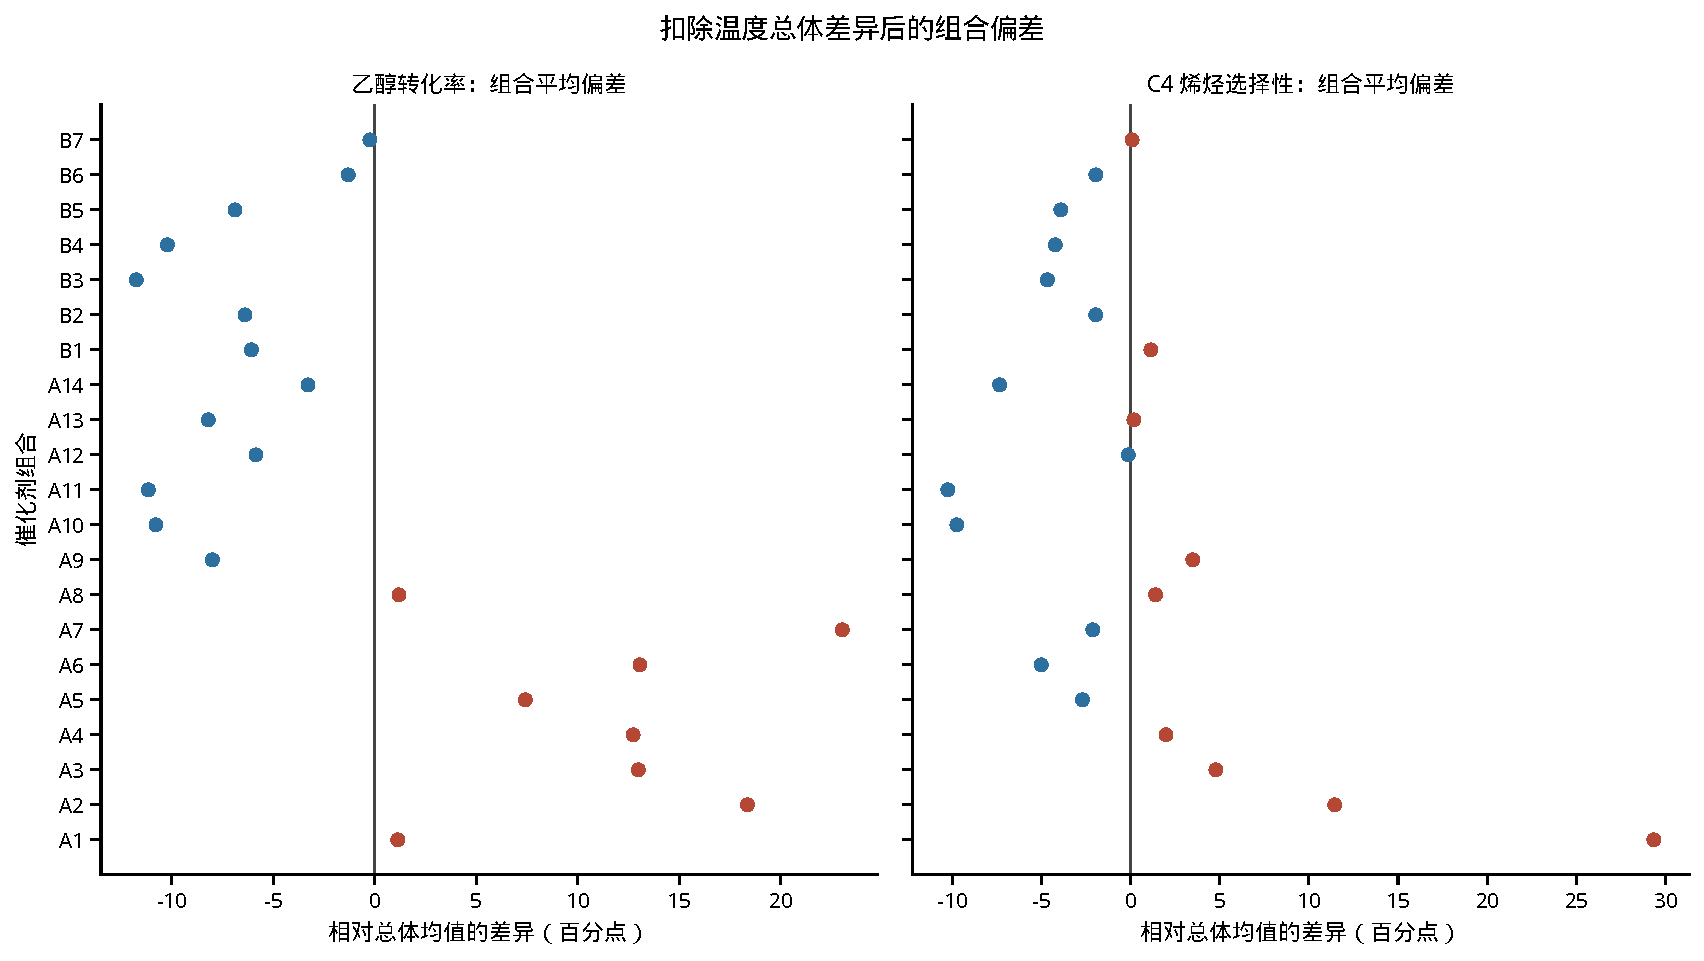
\includegraphics[width=0.94\linewidth]{../../output/q2/figures/01_additive_combination_effects.pdf}
\caption{扣除温度总体差异后的催化剂组合偏差。正值表示该组合跨四个共同温度的平均值
高于总体均值，负值表示低于总体均值。}
\label{fig:q2-combination-effect}
\end{figure}

图中转化率偏差最高的A7比
总体均值高23.043个百分点，最低的B3低11.737个百分点；选择性偏差最高的A1高
29.347个百分点，最低的A11低10.243个百分点。该高低格局与同温排名一致；在扣除
四个温度各自的总体均值差异后，组合之间仍保留数值差别。

\subsubsection{组合与温度的非加和变化}

如果所有组合升温时都增加相同的幅度，那么总体水平、组合偏差和温度偏差三项就足以
还原观测值。式\eqref{eq:q2-residual}中的 \(r_{ij}\) 正是实际值与这一简单还原值的
差；绝对值越大，说明该组合在这个温度下的变化越特殊。由于每个组合—温度条件只有
一次观测，该差值还包含实验误差和未记录因素，不能认定为只由组合与温度共同作用
产生的独立部分。

图\ref{fig:q2-residual}给出每个组合—温度单元未被简单加和结构解释的差值。
\begin{figure}[H]
\centering
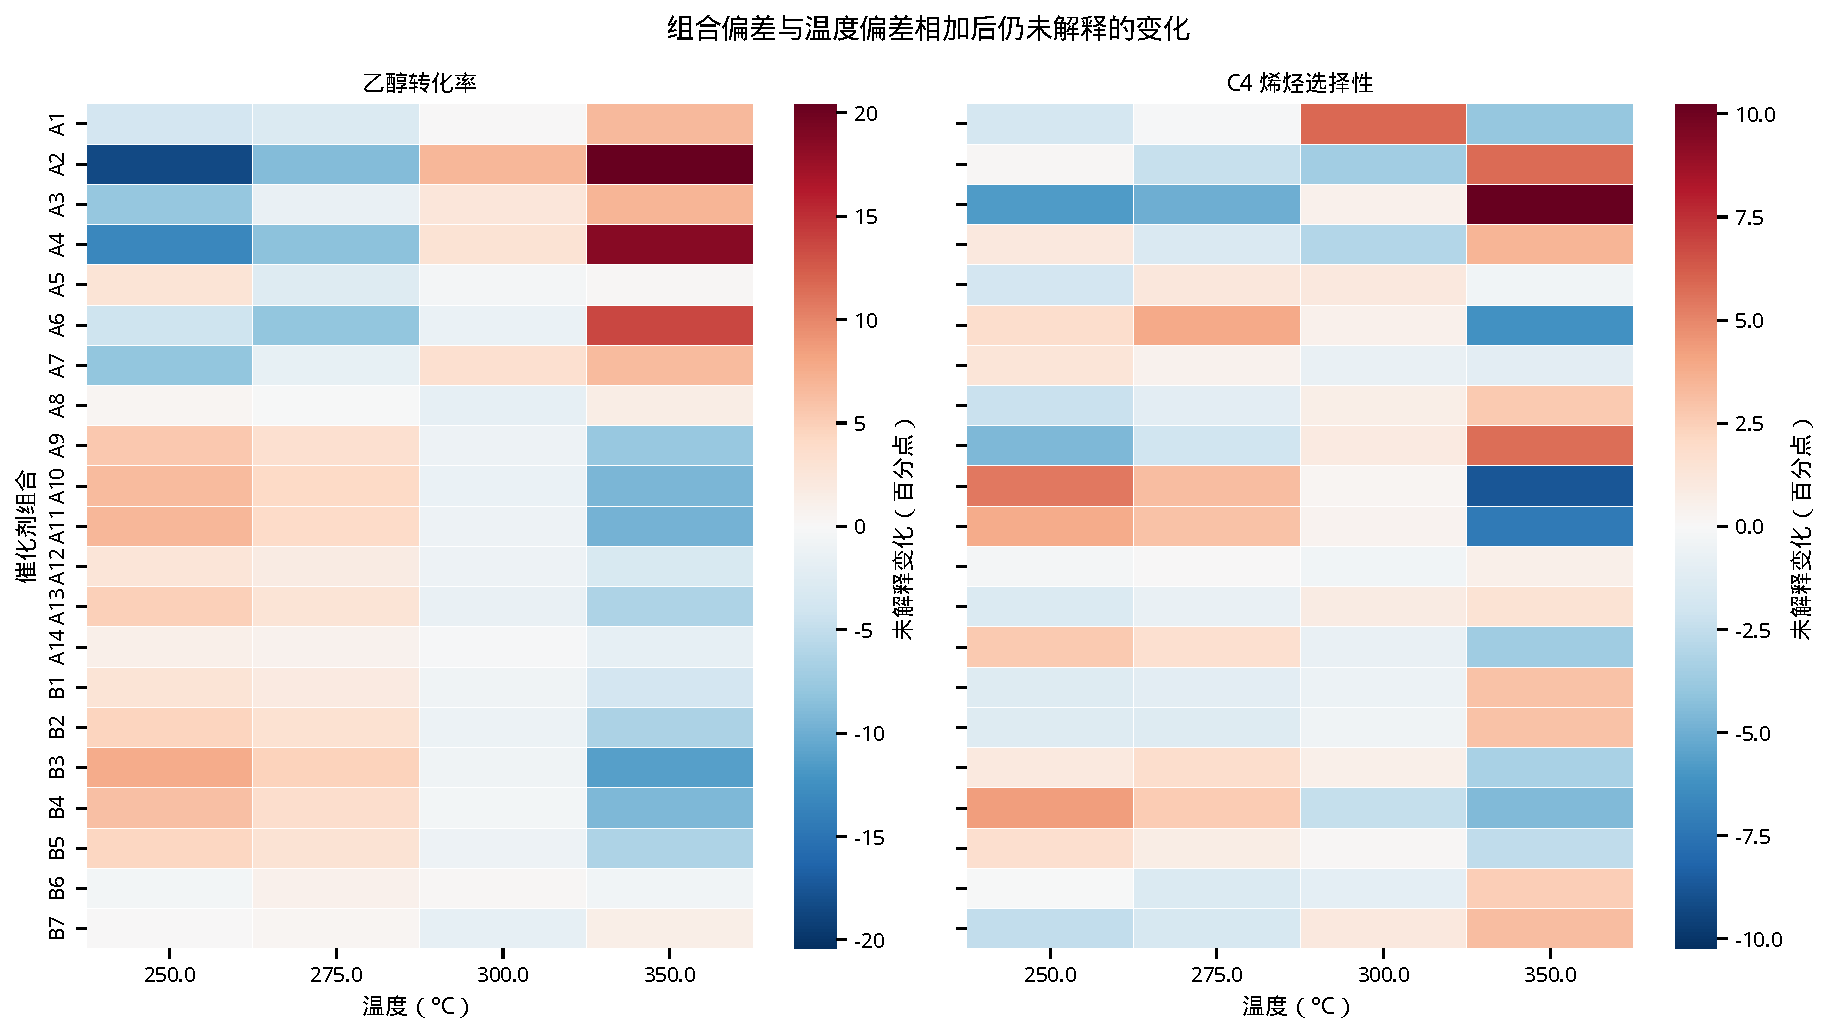
\includegraphics[width=0.90\linewidth]{../../output/q2/figures/03_nonadditive_residual_heatmaps.pdf}
\caption{组合偏差与温度偏差简单相加后仍未解释的单元变化。颜色深浅表示偏离大小，
正负号表示实际值高于或低于加和概括值。}
\label{fig:q2-residual}
\end{figure}

图中转化率偏离最大的单元为A2在350~℃，实际值比加和概括值
高20.441个百分点；选择性偏离最大的单元为A3在350~℃，高10.244个百分点。这说明
不同组合虽然大多随温度上升，但升高幅度并不一致，即组合与温度存在非加和变化迹象。

为比较三类差异的总体大小，分别计算组合偏差、温度偏差和剩余变化的平方和，再除以
84 个观测的总离差平方和。所得比例之和为 1，表示当前数据的差异主要出现在哪一部分，
不表示三个因素各自造成了多少结果。

表\ref{tab:q2-decomposition}比较三类差异在主体数据总离差中的比例。
\begin{table}[H]
\centering
\caption{三类差异占主体数据总差异的比例}
\label{tab:q2-decomposition}
\begin{tabular}{lrrr}
\toprule
考察指标 & 组合间差异 & 温度间差异 & 未解释变化 \\
\midrule
乙醇转化率 & 45.61\% & 38.40\% & 15.99\% \\
C4 烯烃选择性 & 59.69\% & 31.82\% & 8.48\% \\
\bottomrule
\end{tabular}
\end{table}

在当前21种组合和四个共同温度内，两个指标的组合间差异均大于温度间差异；但这一
大小次序是否稳定，还需通过改变组合集合和温度范围检查。

\subsubsection{删除组合或温度后的范围检查}

为检查结论是否依赖某一种组合或某一个温度，两个响应分别进行21次整组删除和4次
整温度删除，共 \(2\times(21+4)=50\) 次结构保持型重新计算。整组删除后每次保留
\(20\times4=80\) 个单元，删除温度后每次保留 \(21\times3=63\) 个单元；这里的50
表示模型复算次数，不是新增实验数或被删除的数据条数。所有删减情形下，两个指标的
跨组合均值仍随温度严格增加；原来排名前五和后五
的组合至少有 80\% 仍留在相应集合中。因此，温度影响的总体方向和主要的高低组合不由
某一个组合或温度单独决定。

但是，``组合间差异大于温度间差异''会随比较范围改变。删除A7后，转化率的组合比例
40.53\%低于温度比例41.24\%；删除A1后，选择性的组合比例34.84\%低于温度比例
51.95\%；删除300~℃后，转化率也出现次序反转。A7和A1分别是对应指标中组合偏差
最大的组合，删除它们会缩小组合间差异；删除一个温度则改变温度范围。所以
表\ref{tab:q2-decomposition}只说明当前 21 种组合和四个温度中的相对大小。

\subsubsection{问题二结论与适用范围}

已有研究表明，乙醇形成较高碳数产物可能经历乙醛生成、缩合、氢转移和脱水等连续步骤，
不同产物路径之间也会相互竞争 \cite{ho2016,moteki2016}。不同催化剂组合可能使这些
步骤对温度的响应不同，从而出现不同的升温幅度。这是与数据相容的一种解释，但文献中
的催化体系与本题并不相同，现有数据也不足以判断具体反应路径或某一种配方成分的作用。

综上，温度影响由同一组合的配对变化回答：升温通常对应更高的转化率和选择性，但
低温段存在少数例外。组合影响由同温排名和扣除温度差异后的组合偏差回答：不同组合
的观测表现存在差异，且两个指标的优势组合不完全相同。非加和剩余进一步表明，不同组合
的升温幅度并不一致。前两项结论较稳定，三类差异的相对大小则依赖纳入的组合和温度
范围；以上关系均限于已测对象和温度，不能作为化学因果作用或未测条件预测。

\FloatBarrier
\subsection{问题三：实测条件推荐与缺测核查}

\subsubsection{收率与实测候选域}

组合 \(i\) 在温度 \(T\) 下的 C4 烯烃收率仍按式\eqref{eq:c4-yield}计算。第三问不拟合连续最优点，
而是在以下两个实测候选域内分别比较收率。

一般情景的实测候选域 \(D_{0}^{\mathrm{all}}\) 包含附件1全部114个组合—温度单元；
严格低温实测候选域为

\begin{equation}
D_{0}^{\mathrm{low}}
=\{(i,T)\in D_{0}^{\mathrm{all}}:T<350~^\circ\mathrm{C}\},
\tag{19}
\label{eq:q3-domain}
\end{equation}

共73个单元。一般情景取 \(D_0=D_{0}^{\mathrm{all}}\)，严格低温情景取
\(D_0=D_{0}^{\mathrm{low}}\)，两种情景分别求

\begin{equation}
(i^*,T^*)=\mathop{\arg\max}_{(i,T)\in D_0}Y_i(T).
\tag{20}
\label{eq:q3-observed-argmax}
\end{equation}

式\eqref{eq:q3-observed-argmax}给出的是附件实测范围内的最高观测收率，不是连续温度
上的全局最优，也不表示未来重复实验中必然仍为第一。

\subsubsection{两种温度情景的推荐结果}

表\ref{tab:q3-recommendations}列出两个实测候选域内的最高收率条件及其与次高值的差距。
\begin{table}[H]
\centering
\caption{两种情景下的实测条件推荐与主要差距}
\label{tab:q3-recommendations}
\begin{tabular}{lrrrr}
\toprule
情景 & 推荐组合 & 温度（℃） & 收率（\%） & 与次高差距（百分点） \\
\midrule
一般情景 & A3 & 400 & 44.7281 & 1.6096 \\
严格低于350~℃ & A2 & 325 & 17.2643 & 6.4716 \\
\bottomrule
\end{tabular}
\end{table}

一般情景的次高单元为A3在450~℃，收率43.1184\%；最高的不同组合为A4在400~℃，
收率36.2778\%，比推荐低8.4502个百分点。因此，一般情景的前两个观测都来自A3，
但A3在450~℃只是单组合个案，不能据此归纳所有组合的高温变化。

严格低温情景的次高单元也是最高的不同组合，即A3在325~℃，收率10.7927\%，比A2
低6.4716个百分点。由于每个条件没有重复实验，这些差距是观测差，而不是统计显著性
结论。

\subsubsection{内部缺测条件的辅助核查}

附件出现的温度标签为250、275、300、325、350、400和450~℃。只有A6--A14、B1和
B2缺少的325~℃同时位于各组合自身实测温度范围内部，共11个单元。本文对每个组合
分别用相邻已测点构造分段三次曲线，并限制曲线不产生与局部数据形态不符的额外振荡；
这种方法称为保形分段三次插值。计算不跨组合借用曲线，不外推，也不搜索标签之间的
任意连续温度。

验证时依次暂时移除一个已知的内部观测，用其余观测预测被移除点，再比较预测值与
真实值；这一操作称为内部遮点。该插值在72次内部遮点中的平均绝对误差为0.7152个
百分点，中位绝对误差为0.1627个
百分点，均低于局部直线的1.5570和0.8092个百分点；72次中有68次误差更小。但它在
5个温度块中只正确识别4次最高候选，最坏遮点误差仍为13.4906个百分点。因此，这一
方法的平均预测偏差和典型预测偏差虽然较小，个别点仍可能出现较大误差。故该方法只
用于缺测核查，预测值不作为观测或正式推荐。

11个缺口中，分段三次插值的最高预测为A7在325~℃的6.5517\%；改用局部直线后，
最高预测为7.2293\%。两者都低于严格低温实测推荐的17.2643\%，故低温推荐不依赖
这两种插值形式中的某一种。完整预测表保留在复现材料中，正文不逐项展开。

\subsubsection{问题三结论与适用范围}

325~℃只有10种组合具有实测值，450~℃只有A3具有实测值，说明附件在高温个案和
低温横向覆盖上都存在限制。遮点误差是预测验证误差，不是实验测量误差；现有无重复
数据也不支持传统显著性检验、置信区间或因果判断。

综上，一般情景推荐A3在400~℃的实测条件，严格低温情景推荐A2在325~℃的实测条件。
对11个已有标签缺口的辅助核查没有发现会改变低温推荐的候选。结论只适用于附件中的
组合和实测温度标签，不能外推到连续温度最优、新配方、工业规模、长期稳定性、安全性
或经济性。

\FloatBarrier
\subsection{问题四：五次补充实验设计}

\subsubsection{由前三问证据缺口确定实验职责}

前三问留下的关键问题不是“模型能否再次得到相同答案”，而是现有数据尚不能回答：
关键高收率区间内部怎样变化、当前最高观测能否复现、领先组合在新增同温条件下是否
仍占优势，以及严格低温边界附近是否存在更高实测条件。下面依次由前三问的证据边界
确定新增实验的职责。

\paragraph{高收率区间的分辨率缺口}

第一问表明，各组合只有5--7个温度点，直线只能概括已测范围内的平均变化，不能确定
局部转折位置。第三问中，A3在350、400和450~℃的实测收率依次为18.0333\%、
44.7281\%和43.1184\%，相邻温度均相差50~℃。因此，现有数据只能把400~℃识别为
最高观测点，不能说明其两侧怎样变化，也不能判断区间内部是否存在更高实测条件。
新增实验需要在350--400~℃和400--450~℃内各补一个温度点。

\paragraph{最高观测的重复性缺口}

附件1的114个组合—温度条件均无独立重复。A3在400~℃的收率虽为当前最高观测值，
却只比其450~℃观测高1.6096个百分点。前三问能够复算并比较这些记录，但无法从单次
观测估计实验波动，也不能判断这一差距能否在相同条件下复现。因此，需要独立重复
A3在400~℃的实验，并直接报告两次观测差。

\paragraph{组合比较的同温证据缺口}

第二问发现不同组合的升温幅度并不一致，因而不能把A3自身区间加密的结果直接解释为
它仍优于其他组合。A3与主要竞争组合A4在350--400~℃之间缺少新增同温观测；若只补测
A3，就无法区分局部优势来自组合差异还是所选温度。为此，需要在同一新增温度下同时
测量A3和A4。

\paragraph{严格低温边界的覆盖缺口}

第三问在 \(T<350~^\circ\mathrm{C}\) 的严格低温情景下推荐A2在325~℃的实测条件，
而A2的下一个观测温度350~℃不满足严格不等式。现有数据因而不能回答325--350~℃之间
是否存在收率更高且仍满足约束的条件。新增实验需要在该开区间内选择一个设备可执行
的温度点。

设新增实验 \(e\) 的催化剂组合和反应温度分别为 \(c_e\) 和 \(T_e\)，新测乙醇
转化率、C4 烯烃选择性和收率分别为 \(X_e,S_e,Y_e\)。每次实验仍按
式\eqref{eq:c4-yield}的同一口径，由 \(X_e\) 与 \(S_e\) 计算 \(Y_e\)。

五次实验均沿用附件1中对应组合的完整配方和装料方式，只改变或重复反应温度，其他
可控条件保持可比。表\ref{tab:q4-design}把上述四类证据缺口落实为五次具体实验；
一次实验可以同时提供区间细化与同温比较信息。

\begin{table}[H]
\centering
\caption{五次补充实验的条件与职责}
\label{tab:q4-design}
\begin{tabular}{clclp{7.0cm}}
\toprule
实验 & 组合 & 温度（℃） & 类型 & 主要职责 \\
\midrule
E1 & A3 & 375   & 新条件 & 细分350--400~℃区间，并与E5作同温比较 \\
E2 & A3 & 425   & 新条件 & 细分400--450~℃区间，判断400~℃附近的高收率区域 \\
E3 & A2 & 337.5 & 新条件 & 细分严格低温情景下的325--350~℃区间 \\
E4 & A3 & 400   & 独立重复 & 检查当前最高观测条件的局部可复现性 \\
E5 & A4 & 375   & 新条件 & 与E1比较，检查A3对竞争组合的局部领先是否保持 \\
\bottomrule
\end{tabular}
\end{table}

A2、A3和A4均采用装料方式I。A2使用200~mg、2~wt\% Co/SiO\(_2\)，200~mg HAP和
1.68~mL/min乙醇条件；A3使用200~mg、1~wt\% Co/SiO\(_2\)，200~mg HAP和
0.9~mL/min乙醇条件；A4使用200~mg、0.5~wt\% Co/SiO\(_2\)，200~mg HAP和
1.68~mL/min乙醇条件。
这些条件均来自附件1，不创造或重组新配方。

\subsubsection{新增观测对既有结论的更新规则}

E1和E2分别与A3已有的350、400、450~℃观测比较。若新增条件取得更高实测收率，则
一般情景推荐相应更新；若没有超过原推荐，它们仍可缩小400~℃两侧的未知区间。
E3严格低于350~℃，若其收率超过A2在325~℃的17.2643\%，则低温推荐更新为
A2在337.5~℃；否则保留原推荐。

设A3在400~℃的原收率为 \(Y_0\)，E4的新测收率为 \(Y_4\)。该条件后续以

\begin{equation}
\overline{Y}_{\mathrm{A3},400}
=\frac{Y_0+Y_4}{2}
\tag{21}
\label{eq:q4-replicate-mean}
\end{equation}

作描述性排序，并同时报告 \(Y_4-Y_0\) 及其绝对值。由于其他条件仍多为单次观测，
式\eqref{eq:q4-replicate-mean}不能用于显著性推断或建立全域误差分布。

E1与E5在375~℃直接比较转化率、选择性和收率。若A4高于A3，只说明A3在这一局部
温度并非始终领先；若A3较高，也不能推广为所有温度下A3均优于A4。这两个新增点不
构成21种组合的共同温度表，因此只补充第二问，不替代其四个共同温度的主体分析。

五次实验完成后，一般情景在全部已有及新增实测条件中重新枚举；严格低温情景只枚举
\(T<350~^\circ\mathrm{C}\) 的实测条件。A3在400~℃按两次观测均值表示，插值预测
不进入实测排序。

\subsubsection{职责充分性与执行边界}

五次实验分别承担一般情景低侧加密、高侧加密、严格低温加密、关键高值复现和竞争组合
同温比较。逐项删除检查表明，删去E1会同时失去350--400~℃加密和同温竞争，删去
E2、E3、E4或E5则分别失去高侧加密、低温加密、局部可复现性检查或竞争组合比较。
因此该方案
在5次预算下职责紧凑，但这不表示所选温度在数学上唯一最优。

若实验结果能够在安排后续实验前获得，可先执行E1--E3，再把第四次用于重复更新后的
A3最高实测条件；第五次在低温推荐发生改变时重复更新后的A2低温最高条件，否则执行
A4在375~℃的实验。该序贯方案只在确有结果反馈权限时适用，不能与表
\ref{tab:q4-design}合并成7次实验。

337.5~℃来自325和350~℃的等距中点。正式执行前须确认设备能够稳定设置该温度；
若设备不支持，必须按真实控温精度重新选择区间内部温度，不能静默舍入后继续声称等距
二分。实验还应记录实际温度、批次和执行顺序，以免把设备或时间漂移误解释为组合差异。

受5次预算限制，该方案不能补齐21种组合在325、375、425或450~℃的完整交叉表，
不能为全部114个原条件增加重复，也不能估计长期失活、全域随机误差或工业放大效应。
这些未覆盖缺口继续构成结论边界；本方案只优先补充最可能改变当前推荐的局部证据。

综上，五次实验由前三问的证据缺口直接推出：第一问确定局部加密和重复位置，第二问
确定竞争组合的同温比较，第三问确定优先细化的两种推荐区域。该设计用于补足决策信息，
不把未来观测预写为结论，也不宣称五次实验足以建立完整响应面或用于证明前三问正确。

\FloatBarrier
\section{模型评价与适用范围}\label{sec:evaluation}

本文没有用一个统一模型强行覆盖四个问题，而是按各问的数据结构选择对应方法。第一问
以组合内相邻观测保留局部变化，并用线性回归概括已测范围内的平均方向；第二问只在
共同温度和匹配组合之间比较，避免把样本构成变化误写成温度或组合影响；第三问把实测
推荐与缺测核查分开；第四问则针对前三问暴露的数据缺口配置有限实验。这样的分工使
每项结论都能回到相应的观测单位和比较范围。

本文采用的检验各有明确边界。独立复算由与主程序分离的计算路径重新读取输入并核对
公式、排序和程序输出，只验证计算一致性；第一问逐点
删除检查平均斜率方向是否受单点支配；第二问整组和整温度删除检查结论对比较对象与
温度范围的依赖；第三问内部遮点衡量缺测估计在已有数据结构中的预测误差；第四问逐项
删除只检查五次实验的职责是否存在冗余。这些检验都不能替代同条件重复、显著性检验或
全域误差估计。

模型的主要限制来自实验设计本身。多数“组合—温度”条件只有一次观测，不同组合的
温度覆盖也不完全相同，故共同温度之外的结果只能作匹配补充或个案说明。附件2又只有
一次时间实验，文献只能提供与现象相容的可能机制，不能证明具体失活路径。

因此，本文结论只适用于附件给出的21种组合、实测温度和观测时段。若要推广到连续温度
最优、新催化剂配方、长期运行、工业规模、安全性或经济性，需要增加重复实验并记录
批次与设备状态，再根据新增数据重新选择曲线形式和误差模型。

\section{结论}\label{sec:conclusion}

针对问题一，21种组合的乙醇转化率和 C4 烯烃选择性在各自已测范围内均呈平均正向关系，
但8种组合至少存在一项局部下降或持平。附件2所给一次350~℃实验中，20---273 min内
转化率和收率总体下降，而 C4 烯烃选择性仅在36.72\%---40.32\%之间波动；该结果只描述
本次实验，不能推广为所有组合的长期稳定性。

针对问题二，同一组合的配对变化表明升温通常对应更高的转化率和选择性，但低温段仍有
少数例外。同温排名和扣除温度总体差异后的组合偏差表明，不同组合的观测表现存在差异；
非加和剩余则显示不同组合的升温幅度并不一致。由于各条件没有独立重复，这些结果属于
描述性比较；组合差异与温度差异的相对大小还会随纳入范围改变，不能解释为显著性结论
或某种配方成分的独立因果作用。

针对问题三，在附件实测条件中，一般情景推荐A3在400~℃，收率为44.7281\%；严格低于
350~℃时推荐A2在325~℃，收率为17.2643\%。对11个内部缺测单元的两种插值核查均未
发现会改变低温推荐的候选，但插值结果不属于实验观测，也不证明连续温度上的全局最优。

针对问题四，安排A3在375~℃和425~℃、A2在337.5~℃、A3在400~℃独立重复以及A4在
375~℃共5次实验。其中，A3的两个新温度补充高收率区域两侧的信息，A2的新温度检查
严格低温边界，A3重复检查当前最高观测的局部可复现性，A3与A4在375~℃形成同温比较。
337.5~℃须以设备能够稳定设置为执行前提；
这5次实验用于弥补关键数据缺口，不预设未来结果，也不足以建立完整响应面。

\begingroup
\sloppy
\begin{thebibliography}{99}
\bibitem{aitchison1982}
Aitchison J. The Statistical Analysis of Compositional Data[J]. Journal of the Royal
Statistical Society: Series B (Methodological), 1982, 44(2): 139--177.

\bibitem{ho2016}
Ho C R, Shylesh S, Bell A T. Mechanism and Kinetics of Ethanol Coupling to Butanol
over Hydroxyapatite[J]. ACS Catalysis, 2016, 6(2): 939--948.
DOI: 10.1021/acscatal.5b02672.

\bibitem{moteki2016}
Moteki T, Flaherty D W. Mechanistic Insight to C--C Bond Formation and Predictive
Models for Cascade Reactions among Alcohols on Ca- and Sr-Hydroxyapatites[J].
ACS Catalysis, 2016, 6(7): 4170--4183.

\bibitem{sushkevich2017}
Sushkevich V L, Ivanova I I. Mechanistic Study of Ethanol Conversion into Butadiene
over Silver Promoted Zirconia Catalysts[J]. Applied Catalysis B: Environmental, 2017,
215: 36--49.

\bibitem{yan2018}
Yan T T, Yang L, Dai W L, et al. On the Deactivation Mechanism of Zeolite Catalyst
in Ethanol to Butadiene Conversion[J]. Journal of Catalysis, 2018, 367: 7--15.

\bibitem{searle1980}
Searle S R, Speed F M, Milliken G A.
Population marginal means in the linear model: an alternative to least squares means[J].
The American Statistician, 1980, 34(4): 216--221.

\bibitem{nisttwoway}
National Institute of Standards and Technology.
Two-way crossed ANOVA[EB/OL].
\url{https://www.itl.nist.gov/div898/handbook/prc/section4/prc437.htm},
2026-07-29.

\bibitem{graphpadnorep}
GraphPad Software.
Two-way ANOVA without replication[EB/OL].
\url{https://www.graphpad.com/guides/prism/latest/statistics/stat_when-there-is-no-replication.htm},
2026-07-29.

\bibitem{nistreplication}
National Institute of Standards and Technology.
Testing model adequacy requires replicate measurements[EB/OL].
\url{https://www.itl.nist.gov/div898/handbook/pmd/section4/pmd446.htm},
2026-07-30.

\bibitem{nistrsmcompare}
National Institute of Standards and Technology.
Comparisons of response surface designs[EB/OL].
\url{https://www.itl.nist.gov/div898/handbook/pri/section3/pri3363.htm},
2026-07-30.
\end{thebibliography}
\endgroup


\end{document}
